\documentclass[aspectratio=1610]{beamer}
\usepackage[T1]{fontenc}

\usetheme{wildcat}


\title{GA-SARIMA}
\date{7 de mayo de 2025}
\author{Heriberto Espino Montelongo}



\begin{document}

\begin{frame}
\titlepage
\end{frame}

% \begin{frame}{Table of Contents}
%     \tableofcontents
% \end{frame}



\begin{frame}{Tesis Central}
La modelación SARIMA es un enfoque clásico y ampliamente aceptado para series temporales estacionarias con estacionalidad estructurada. Sin embargo, su desempeño depende críticamente de una adecuada selección de hiperparámetros $(p,d,q)(P,D,Q)_s$, que comúnmente se realiza mediante inspección de las autocorrelaciones simiples y parciales significativas. Esta metodología, aunque efectiva en entornos simples, se vuelve subóptima frente a datos reales caracterizados por múltiples escalas temporales, ruido estructurado, patrones no lineales y efectos estacionales complejos.
\end{frame}

\begin{frame}{Tesis Central}
Frente a estas limitaciones, los algoritmos genéticos (GA) surgen como una alternativa. Estas técnicas evolutivas permiten una exploración del espacio de soluciones a través de operadores de selección, crossover y mutación. Aplicados a la identificación de modelos SARIMA, los GA maximizan funciones objetivo como AIC, BIC, MAPE o RMSPE.
\end{frame}

\begin{frame}{Tesis Central}
Los métodos clásicos de estimación como la Máxima Verosimilitud (MLE) o Mínimos Cuadrados (OLS) proporcionan soluciones óptimas bajo supuestos ideales, pero presentan limitaciones prácticas cuando la función de verosimilitud es multimodal, no diferenciable o se enfrenta a datos ruidosos o no lineales. En estos escenarios, un GA puede saltarse mínimos locales y buscar soluciones más adecuadas para la estructura de la serie.
\end{frame}

\begin{frame}{Tesis Central}
\textbf{Tesis:} La combinación de algoritmos genéticos con modelación SARIMA permite superar las limitaciones de los métodos clásicos de identificación y estimación, mejorando la precisión de predicción.
\end{frame}


\section{Algoritmos Genéticos (GA)}
\begin{frame}{Algoritmos Genéticos}
\begin{itemize}
  \item \textbf{Definición:} métodos evolutivos de búsqueda aleatoria.
  \item \textbf{Operadores:}
  \begin{itemize}
    \item Selección.
    \item crossover (crossover).
    \item Mutación.
  \end{itemize}
  \item \textbf{Etapas del algoritmo:}
  \begin{enumerate}
    \item Inicialización aleatoria.
    \item Evaluación por función de aptitud.
    \item Selección, crossover y mutación iterativos.
    \item Eliminación de soluciones no aptas.
    \item Repetición hasta convergencia o límite de generaciones
  \end{enumerate}
\end{itemize}
\end{frame}


\section{Modelo SARIMA}
\begin{frame}{Modelo SARIMA}
    Se representa como: \textbf{SARIMA($p,d,q$)($P,D,Q$)\textsubscript{s}}.

  \begin{equation*}
    \phi_p(B) \Phi_P(B^s) \nabla^d \nabla^D_s X_t = \theta_q(B) \Theta_Q(B^s) \epsilon_t
  \end{equation*}
\end{frame}




\begin{frame}{Criterios de Selección del Modelo}
  \begin{itemize}
    \item \textbf{Akaike Information Criterion (AIC):}
      \[
        \text{AIC} = -2 \log(L) + 2k
      \]
    \item \textbf{Bayesian Information Criterion (BIC):}
      \[
        \text{BIC} = -2 \log(L) + k \log(n)
      \]
  \end{itemize}
  Donde $L$ es la verosimilitud, $k$ el número de parámetros y $n$ el tamaño de muestra.

\end{frame}




\begin{frame}{Criterios de Selección de Parámetros}
\begin{itemize}
    \item \textbf{Error porcentual absoluto medio (MAPE):}
\begin{equation*}
\text{MAPE} = \frac{1}{m - 1} \sum_{l=2}^{m} \left| \frac{y_0(l) - z_0(l)}{y_0(l)} \right| \times 100\%
\end{equation*}

\item \textbf{Raíz del error cuadrático medio porcentual (RMSPE):}
\begin{equation*}
\text{RMSPE} = \sqrt{ \frac{1}{m - 1} \sum_{l=2}^{m} \left( \frac{y_0(l) - z_0(l)}{y_0(l)} \right)^2 } \times 100\%
\end{equation*}
\end{itemize}

Son funciones objetivo para evaluar precisión.
\end{frame}







\section{Enfoque GA–SARIMA}



\begin{frame}[fragile]
    \frametitle{GA-SARIMA Paralelo}
    \begin{figure}
        \centering
        \includegraphics[width=0.8\textwidth]{Screenshot 2025-05-06 183127.png}
    \end{figure}
\end{frame}








\begin{frame}[fragile]
    \frametitle{Ilustración}
    \begin{figure}
        \centering
        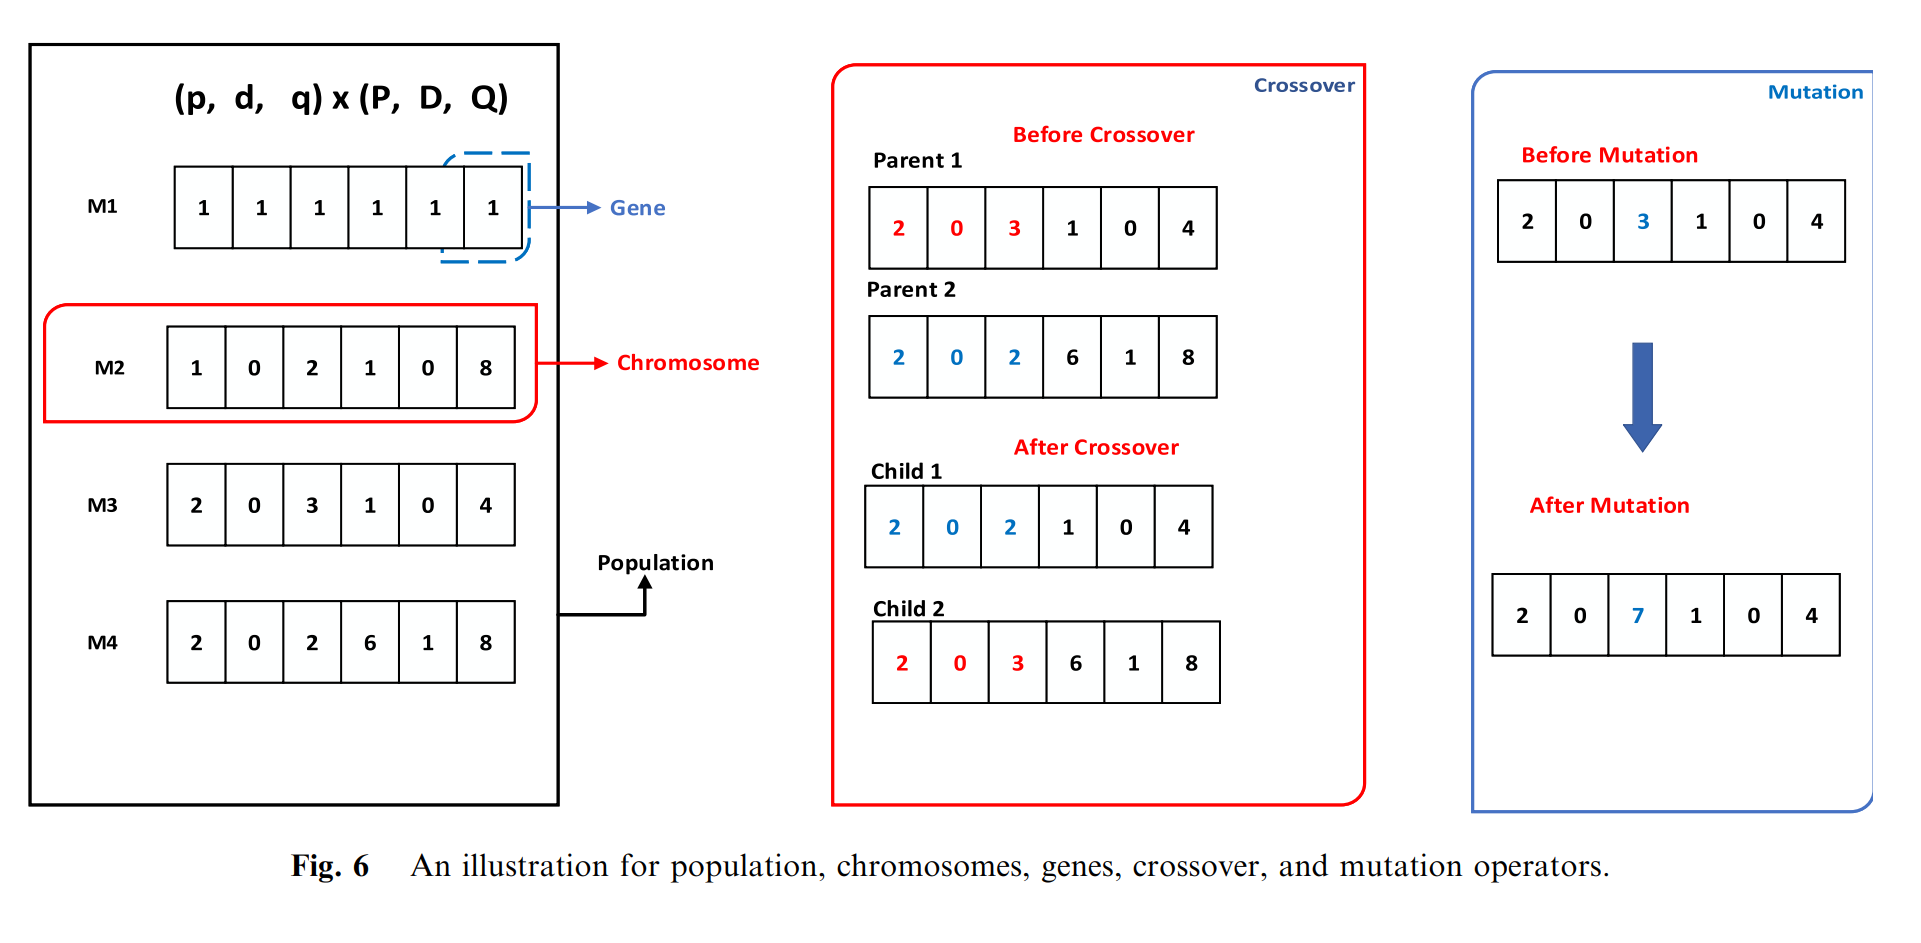
\includegraphics[width=0.95\textwidth]{Opti-Imagenes/02-04.png}
    \end{figure}
\end{frame}



\begin{frame}{Esquema Básico del Algoritmo Genético}
\begin{itemize}
  \item \textbf{Inicialización:} se genera aleatoriamente una población inicial de tamaño \(N\), promoviendo diversidad.
  \item \textbf{Función de Fitness:} se utiliza el criterio AIC para seleccionar el mejor modelo SARIMA.
  \item \textbf{Selección:} individuos con menor AIC tienen mayor probabilidad de reproducción.
  \item \textbf{Crossover:} combinación de pares de soluciones para explorar nuevas regiones del espacio.
  \item \textbf{Mutación:} pequeñas alteraciones aleatorias para mantener diversidad y evitar óptimos locales.
  \item \textbf{Criterio de Paro:} el algoritmo se detiene tras cierto número de generaciones o si no hay mejora significativa.
\end{itemize}
\end{frame}





\begin{frame}[fragile]
    \frametitle{Flujo de Trabajo para Parámetros}
    \begin{figure}
        \centering
        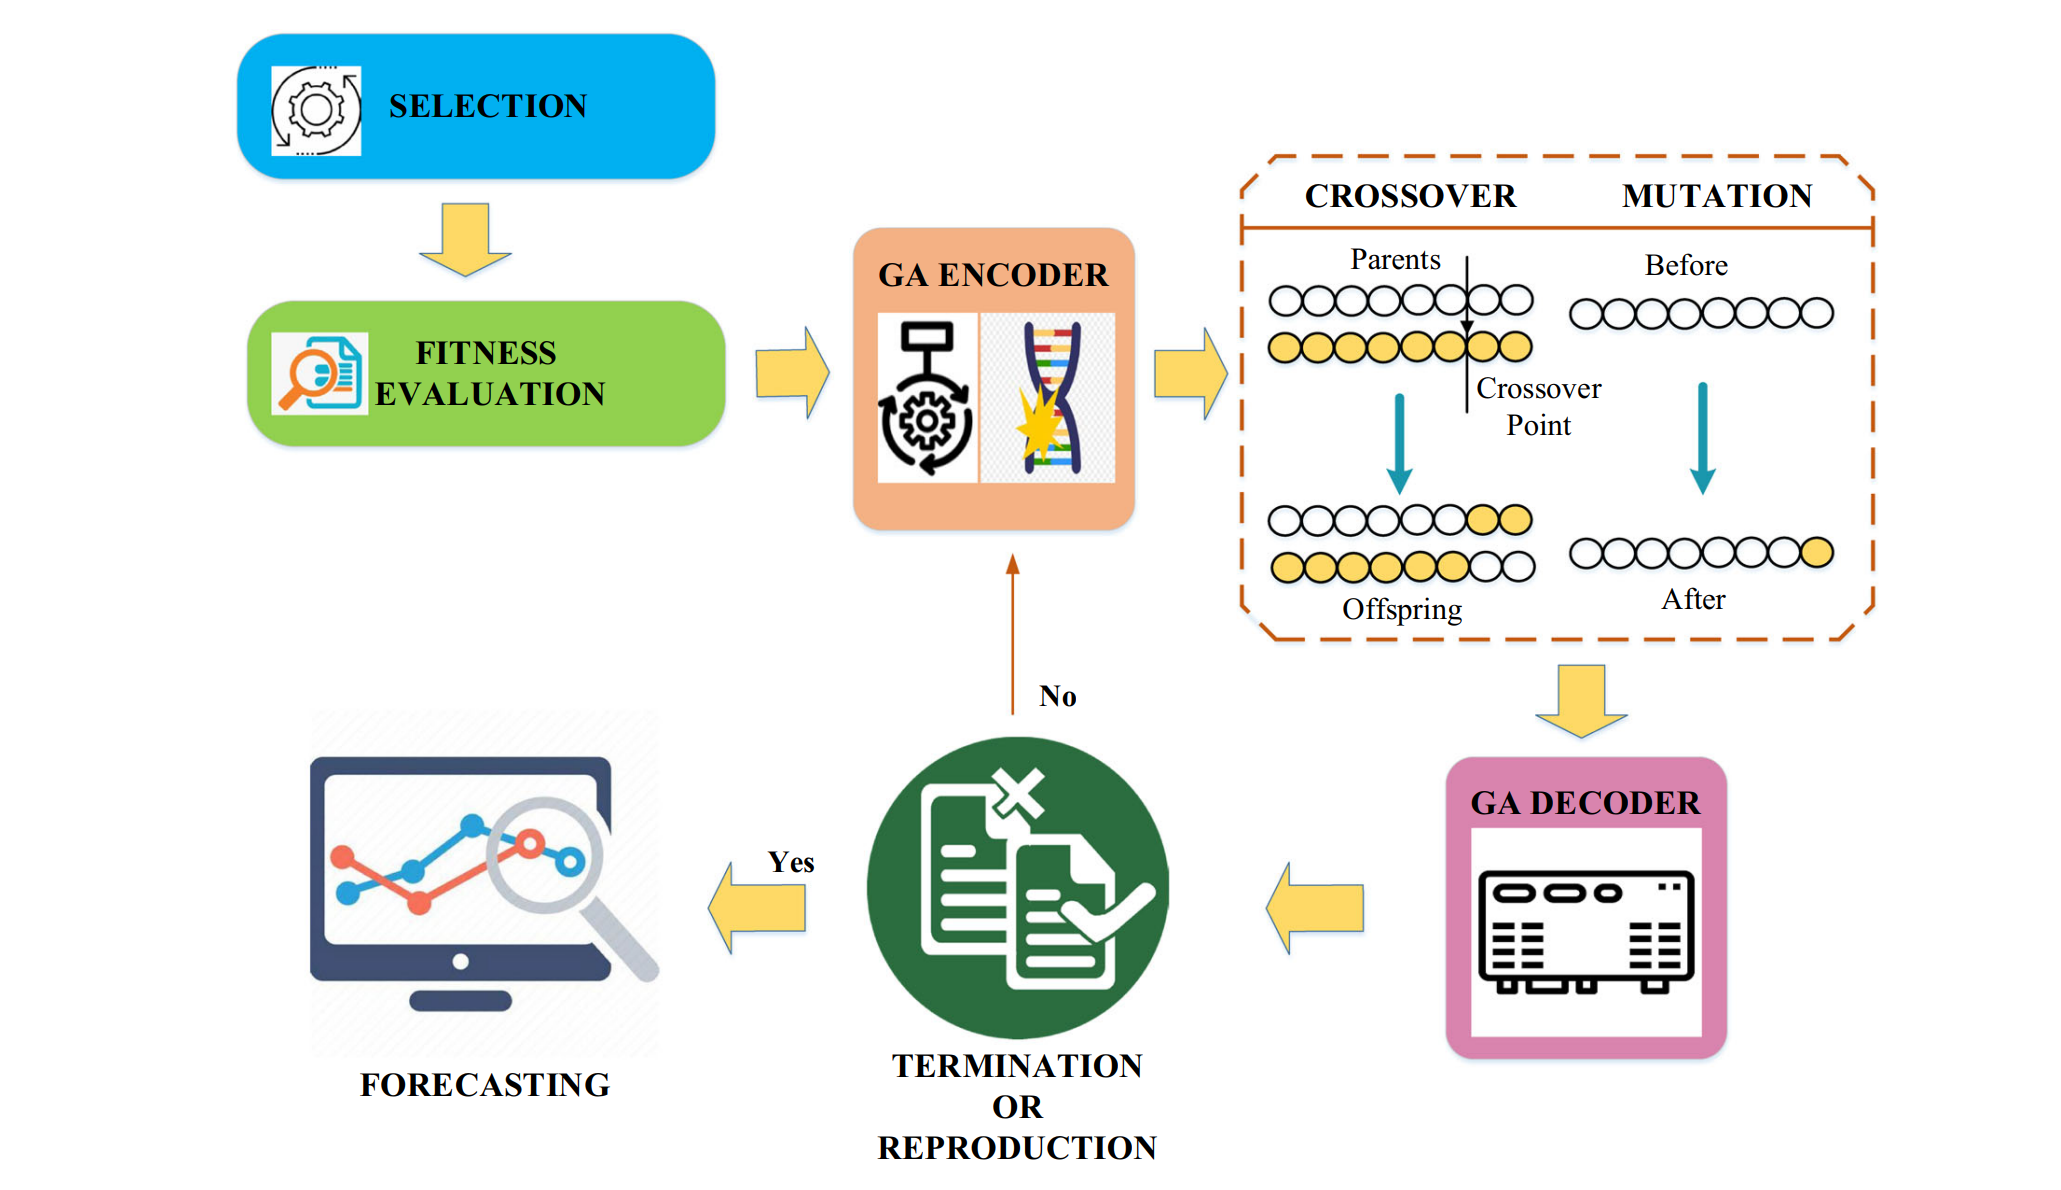
\includegraphics[width=1\textwidth]{Opti-Imagenes/01-02.png}
    \end{figure}
\end{frame}






\begin{frame}{Para los Parámetros}
\begin{itemize}
    \item Los parámetros (genes) se representan como cadenas binarias.
    \item La decodificación es el proceso de convertir esas cadenas en números reales dentro de un rango.
\end{itemize}


\[
y = y_{\text{LOW}} + \frac{y_{\text{DEC}}}{2^m - 1}(y_{\text{UPR}} - y_{\text{LOW}})
\]

\begin{itemize}
    \item \( y \): valor real decodificado.
    \item \( y_{\text{DEC}} \): valor decimal de la cadena binaria.
    \item \( m \): número de bits.
    \item \( y_{\text{LOW}}, y_{\text{UPR}} \): cota inferior y superior del rango.
\end{itemize}
\end{frame}




























\section{Resultados}


\begin{frame}[fragile]
    \frametitle{Fuerza Bruta}
    \begin{figure}
        \centering
        \includegraphics[width=1\textwidth]{Opti-Imagenes/03-02.png}
    \end{figure}
\end{frame}


\begin{frame}[fragile]
    \frametitle{Algoritmos Genéticos}
    \begin{figure}
        \centering
        \includegraphics[width=1\textwidth]{Opti-Imagenes/03-01.png}
    \end{figure}
\end{frame}






\begin{frame}[fragile]
    \frametitle{Curva de Aprendizaje}
    \begin{figure}
        \centering
        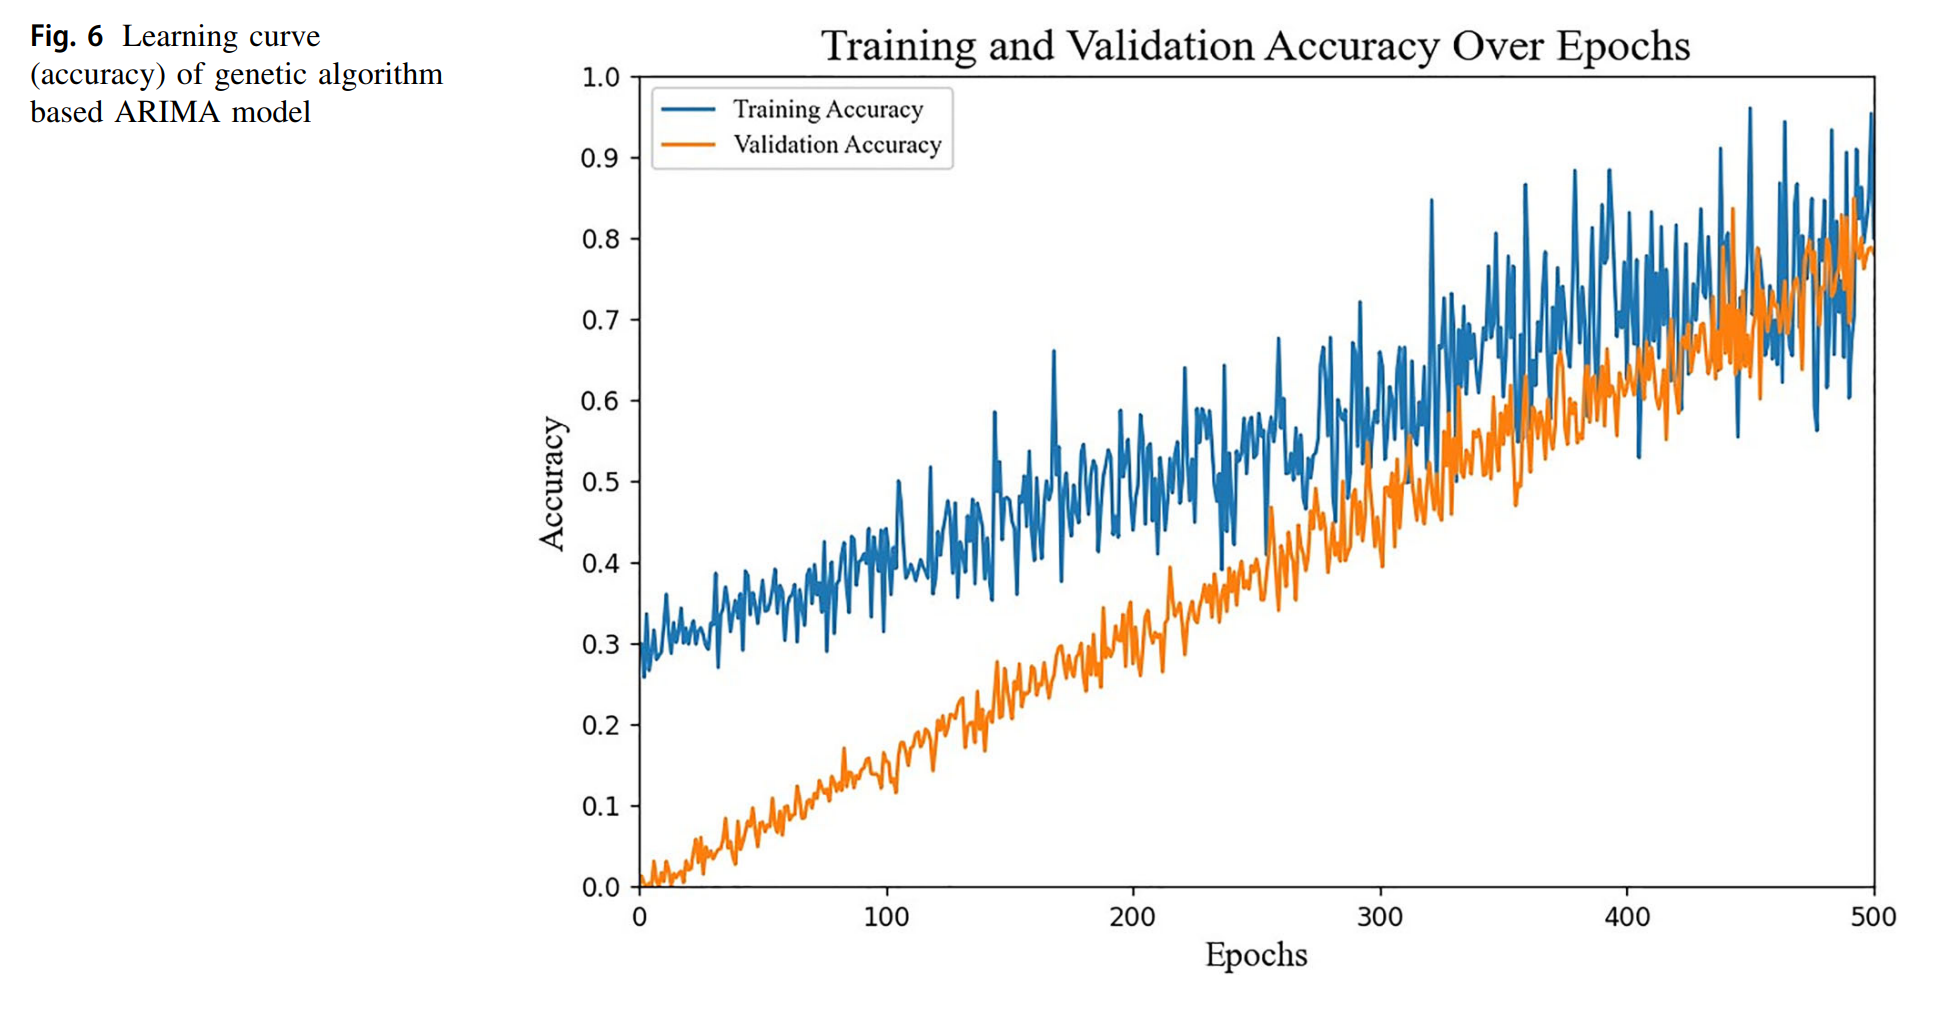
\includegraphics[width=1\textwidth]{Opti-Imagenes/01-03.png}
    \end{figure}
\end{frame}



    
\begin{frame}[fragile]
    \frametitle{Curva de Pérdida}
    \begin{figure}
        \centering
        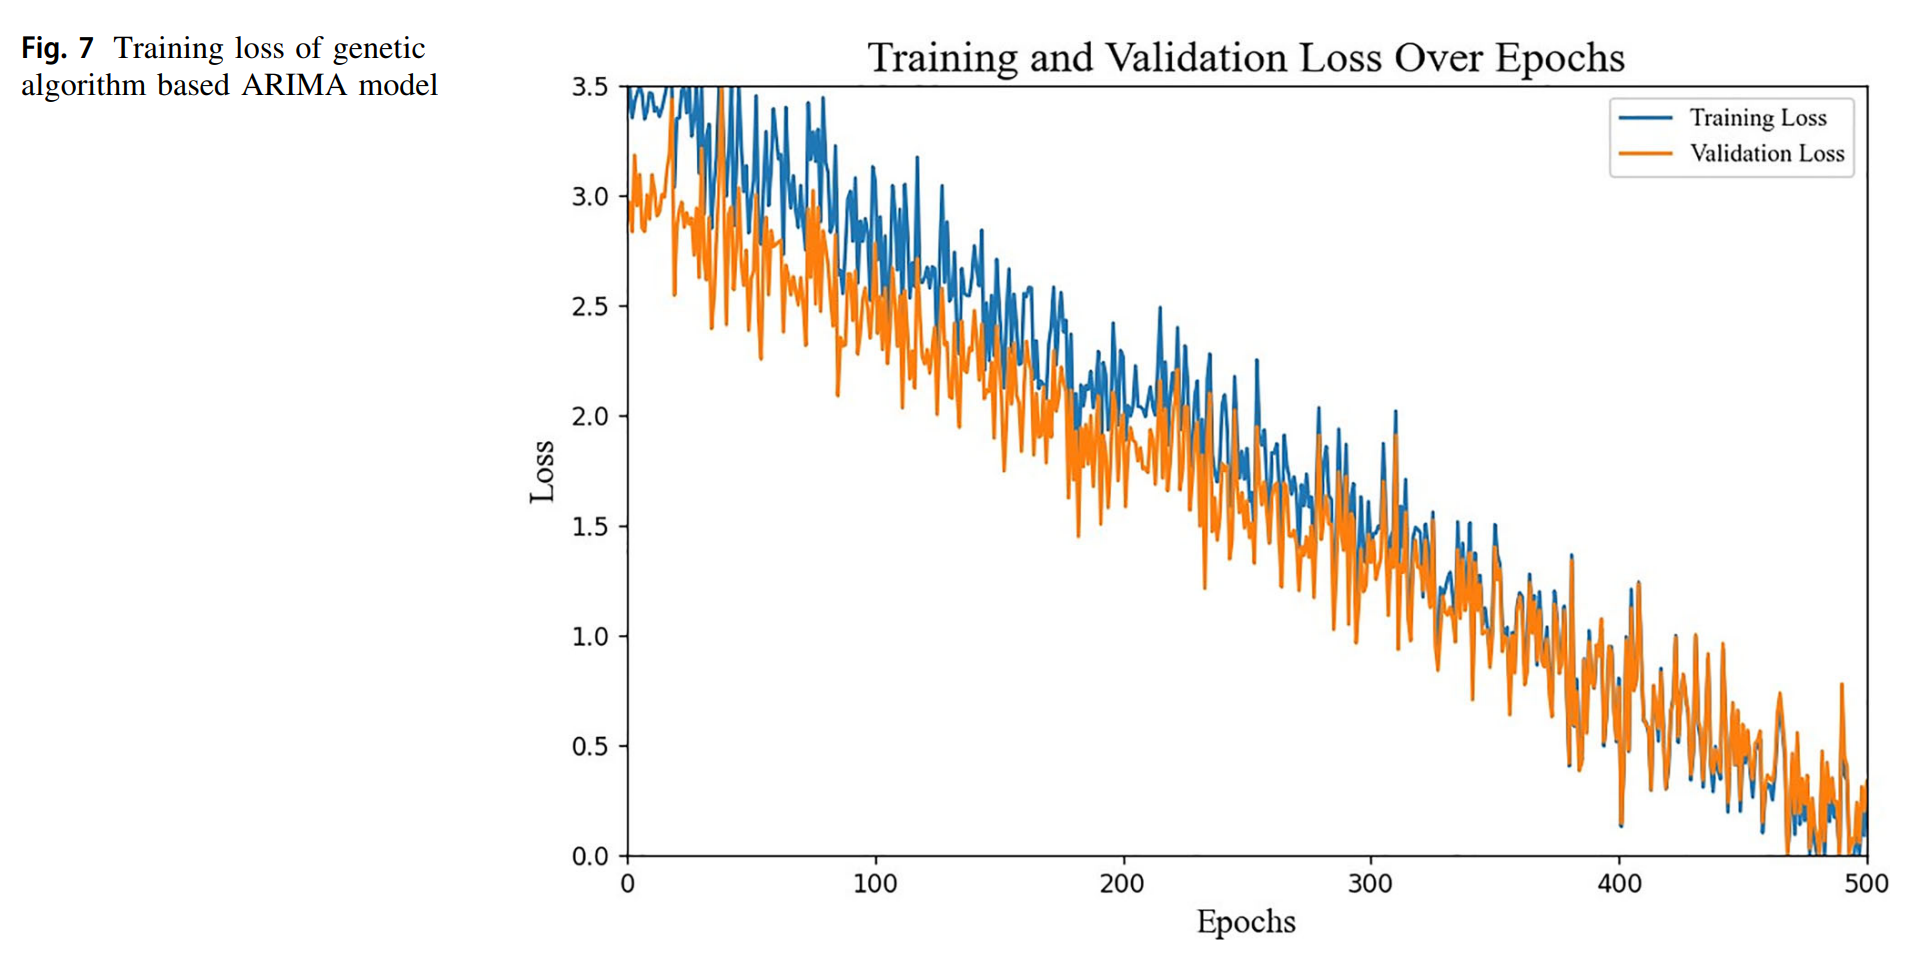
\includegraphics[width=1\textwidth]{Opti-Imagenes/01-04.png}
    \end{figure}
\end{frame}

































% Diapositiva 4: Tabla Comparativa
\begin{frame}{Tabla Comparativa de Modelos}
  \begin{table}[ht]
    \centering
    \scriptsize
    \begin{tabular}{@{}lcccccc@{}}
      \toprule
      \textbf{Modelo} & \textbf{MAE} & \textbf{RMSE} & \textbf{RRSE} & \textbf{RAE} & \textbf{MSE} & \textbf{R²} \\
      \midrule
      Hybrid RL-RF {\footnotesize (2023)} & 3.45 & 1.45 & 0.78 & 2.49 & 2.50 & 1.78 \\
      ANN {\footnotesize (2023)}            & 1.75 & 3.48 & 0.75 & 1.68 & 2.75 & 3.12 \\
      Deep Q-Learning {\footnotesize (2023)}& 0.99 & 2.79 & 0.45 & 1.67 & 3.75 & 2.79 \\
      SVM {\footnotesize (2023)}            & 1.48 & 0.76 & 0.55 & 3.49 & 2.79 & 1.70 \\
      Decision Trees {\footnotesize [22]}   & 0.48 & 3.49 & 1.48 & 3.47 & 2.49 & 1.79 \\
      \midrule
      GA-ARIMA                 & 0.80 & 3.75 & 1.21 & 0.82 & 0.07 & 0.54 \\
      Reinforced RF             & 1.28 & 2.48 & 0.54 & 0.91 & 0.55 & 0.90 \\
      \bottomrule
    \end{tabular}
  \end{table}
  {\footnotesize (Yunli, 2023; Thangavel et al., 2023; Sharafi et al., 2023; Baswaraju et al., 2023; Kolipaka \& Namburu, 2023)}
\end{frame}

\begin{frame}[fragile]
    \frametitle{Métricas de Evaluación}
    \begin{figure}
        \centering
        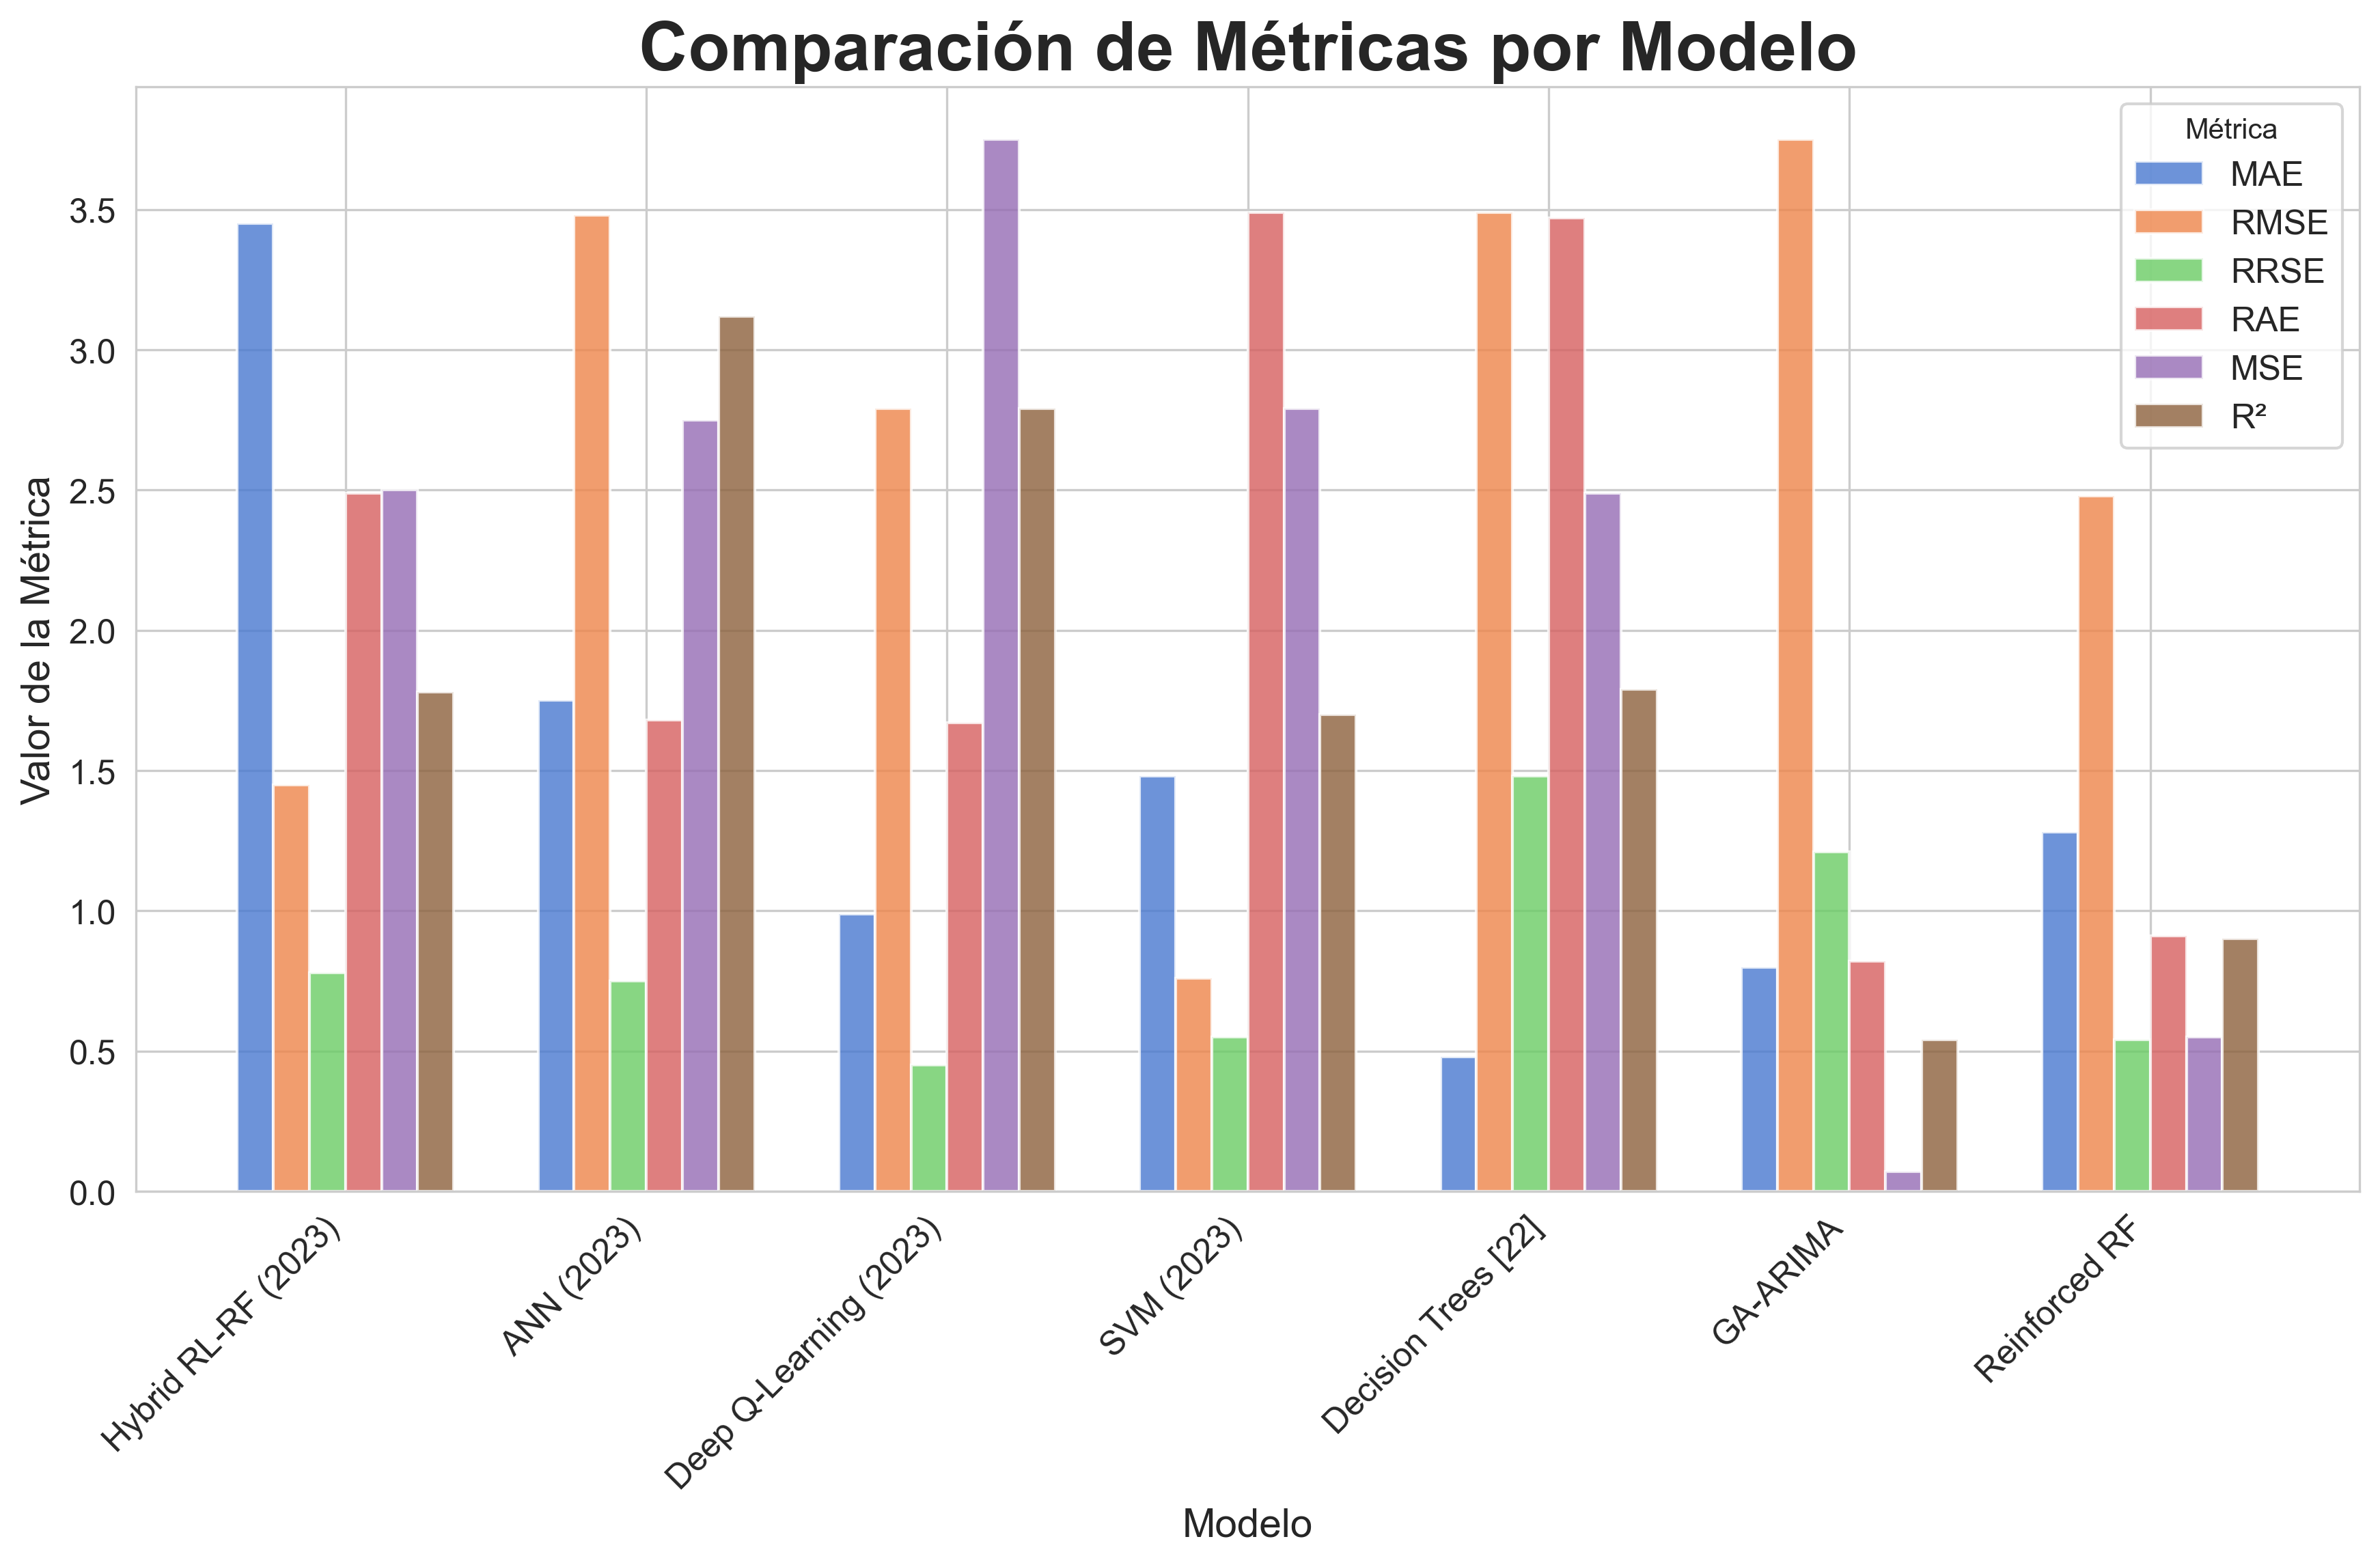
\includegraphics[width=0.8\textwidth]{Opti-Imagenes/comparacion_metricas_modelos.png}
    \end{figure}
\end{frame}






































\section{Tiempos de Ejecución}

\begin{frame}[fragile]
    \frametitle{Tiempos de Ejecución para Distintos Hiperparámetros}
    \begin{figure}
        \centering
        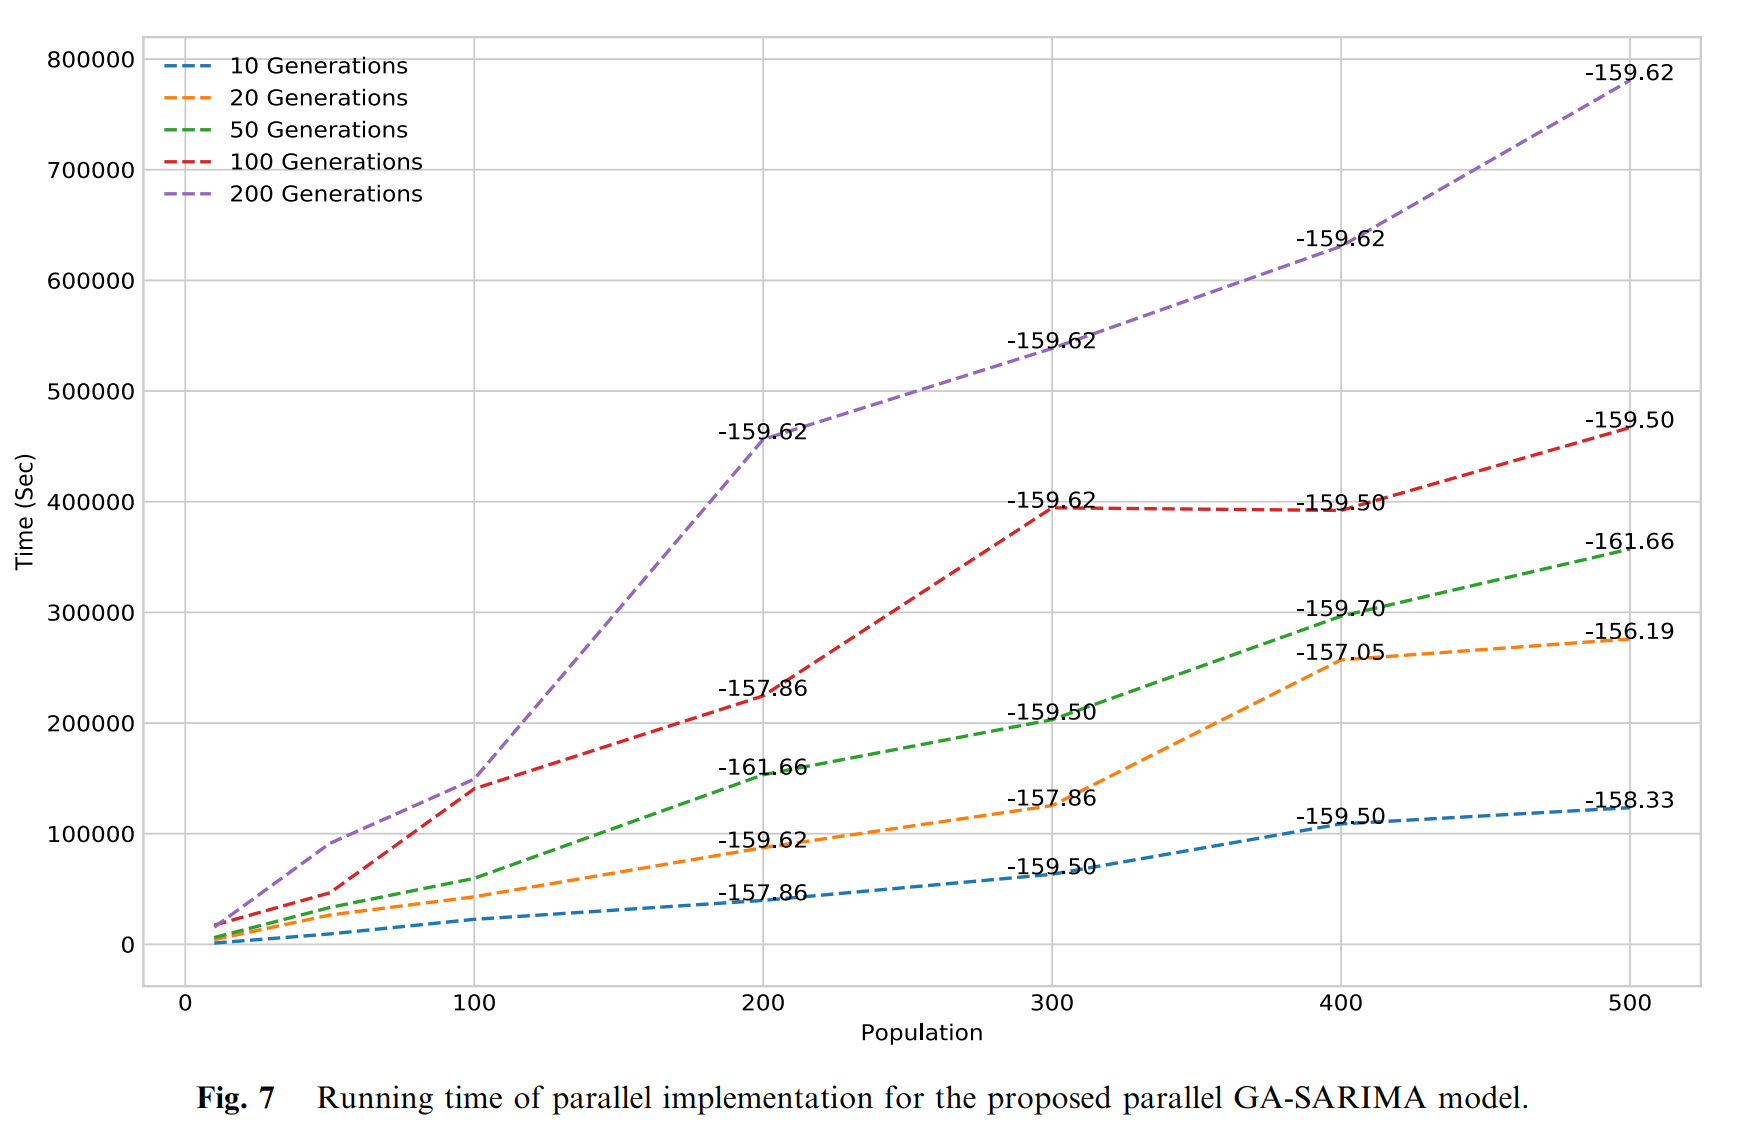
\includegraphics[width=1\textwidth]{Opti-Imagenes/02-05.png}
    \end{figure}
\end{frame}

% Diapositiva 1: Tabla de tiempos
\begin{frame}{Tiempos de Ejecución de Modelos en Parámetros}
  \begin{table}[ht]
    \centering
    \scriptsize
    \begin{tabular}{@{}lcc@{}}
      \toprule
      \textbf{Modelo} & \textbf{Tiempo (s)} & \textbf{Referencia} \\
      \midrule
      Polynomial Regression & 4.56786 & Panigrahi et al. (2023) \\
      Reinforcement Learning & 3.94585 & Boori et al. (2023) \\
      Gradient Boosting & 2.35498 & Torsoni et al. (2023) \\
      Artificial Neural Network & 5.76832 & Sharafi et al. (2023) \\
      GA-ARIMA  & 2.12488 & \\
      Reinforced RF  & 3.35763 & \\
      \bottomrule
    \end{tabular}
  \end{table}
\end{frame}

\begin{frame}[fragile]
    \frametitle{Tiempo Computacional}
    \begin{figure}
        \centering
        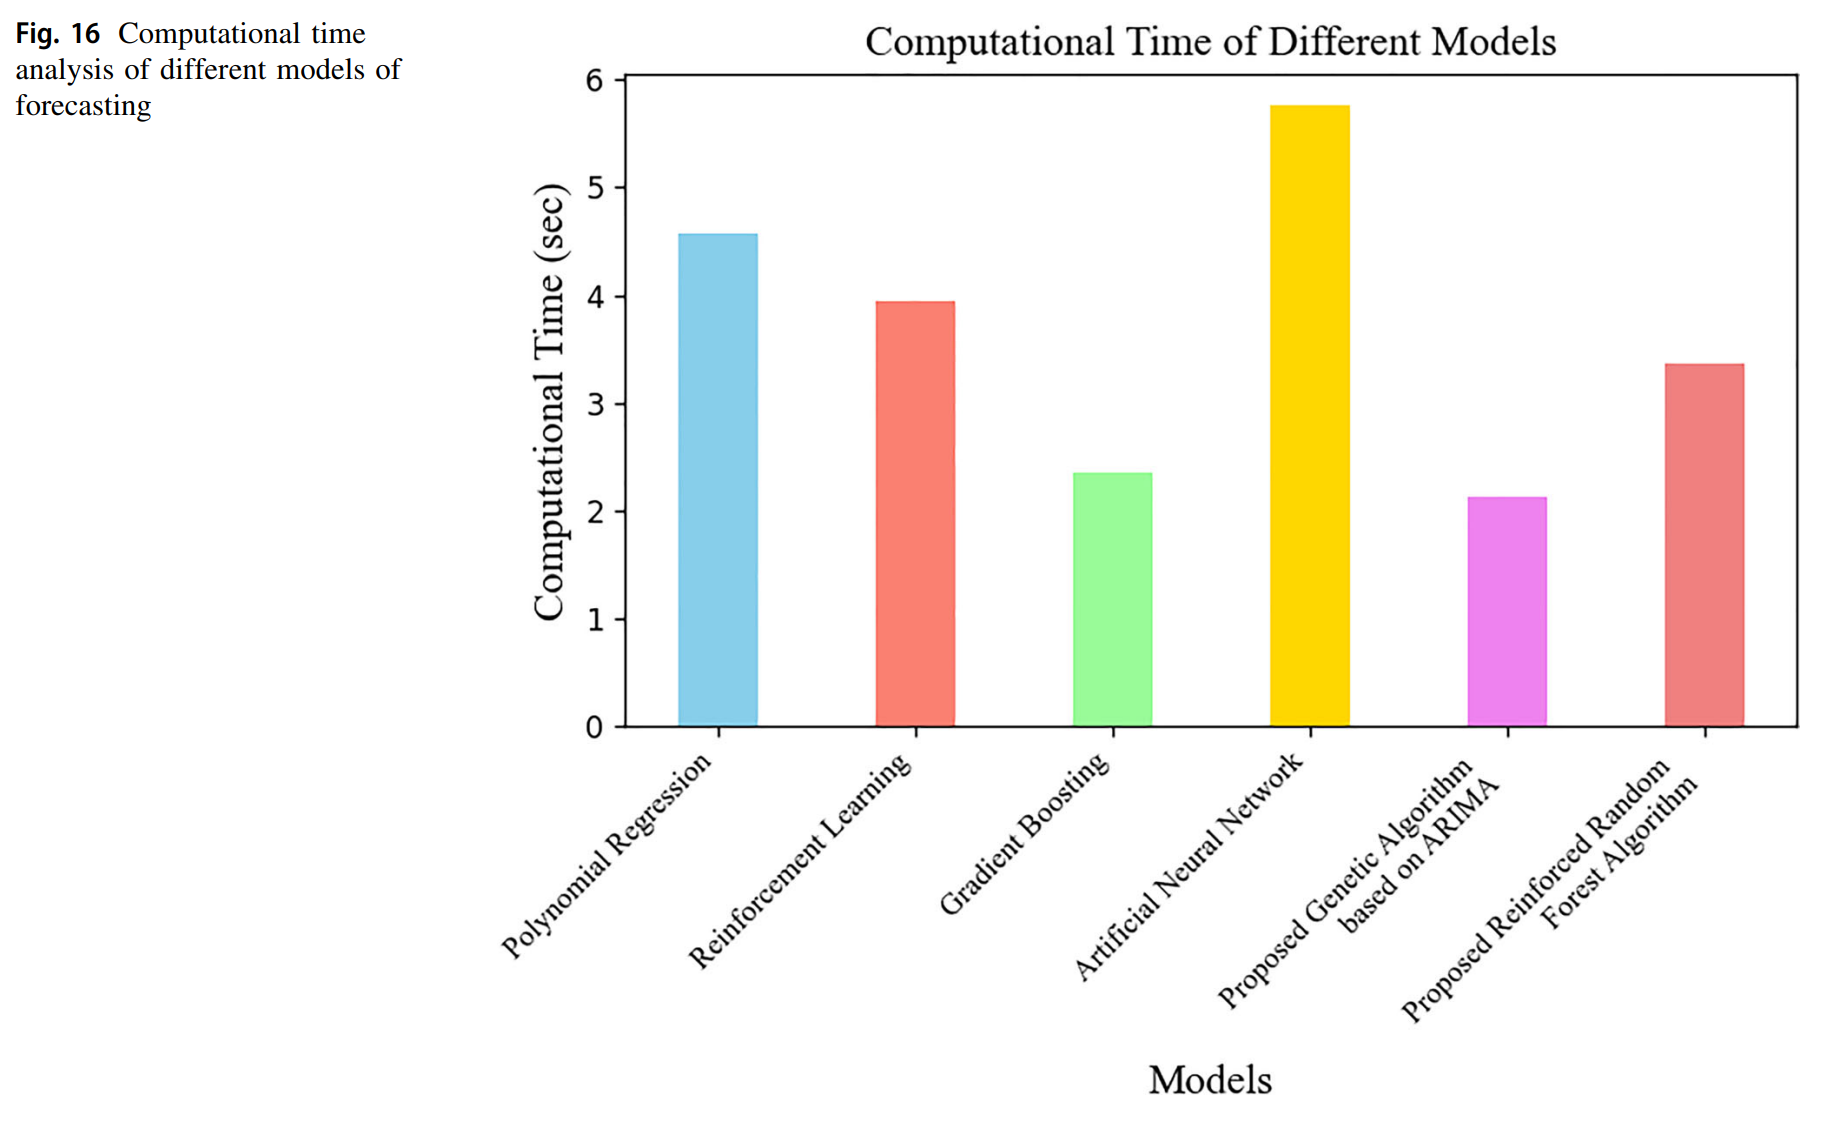
\includegraphics[width=1\textwidth]{Opti-Imagenes/01-08.png}
    \end{figure}
\end{frame}











% Diapositiva 1: Tabla de tiempos
\section{Conclusiones}






% Sección 6






















































\begin{frame}{Conclusión}
\begin{itemize}
    \item Los métodos clásicos como ARIMA presentan limitaciones importantes en la predicción, debido a:
    \begin{itemize}
        \item Dificultad en el reconocimiento de patrones complejos.
        \item Problemas en la determinación óptima de los retardos (lags).
    \end{itemize}
    \item El uso de algoritmos genéticos mejora los resultados utilizando múltiples poblaciones y seleccionando los mejores individuos.
    \item Dado el elevado número de parámetros en SARIMA, su capacidad predictiva se ve limitada. El GA ofrece una forma confiable de estimar sus hiperparámetros. Se concluye que el modelo GA-SARIMA es una alternativa robusta para estimar los hiperparámetros \((p,d,q)(P,D,Q)_s\).
    \item Líneas futuras de investigación:
\end{itemize}
\end{frame}

\begin{frame}{Implementación}
  \begin{itemize}
      \item En aplicaciones con restricción de tiempo, preferir GA-ARIMA o Gradient Boosting.  
      \item Modelos de rango medio (Reinforced RF, RL) equilibran velocidad y
flexibilidad
      \item Métodos más complejos (ANN, Polynomial Regression) requieren mayor
potencia computacional.
Selección del modelo debe considerar tiempo de cómputo junto con
precisión.
  \end{itemize}
\end{frame}






\begin{frame}{Referencias}
\begin{itemize}
    \item Farsi, M., Hosahalli, D., Manjunatha, B. R., Gad, I., Atlam, E.-S., Ahmed, A., Elmarhomy, G., Elmarhoumy, M., & Ghoneim, O. A. (2021). Parallel genetic algorithms for optimizing the SARIMA model for better forecasting of the NCDC weather data. \textit{Alexandria Engineering Journal, 60(1), 1299–1316}. https://doi.org/10.1016/j.aej.2020.10.052
    \item  Guo, Y. (2024). Integrating genetic algorithm with ARIMA and reinforced random forest models to improve agriculture economy and yield forecasting. \textit{Soft Computing, 28, 1685–1706}. https://doi.org/10.1007/s00500-023-09516-8 
\end{itemize}
\end{frame}









\standout{Gracias}



\end{document}